% !TEX root = hazelnut-dynamics.tex

\begin{figure}[t]
\begin{subfigure}[t]{0.65\textwidth}
\centering
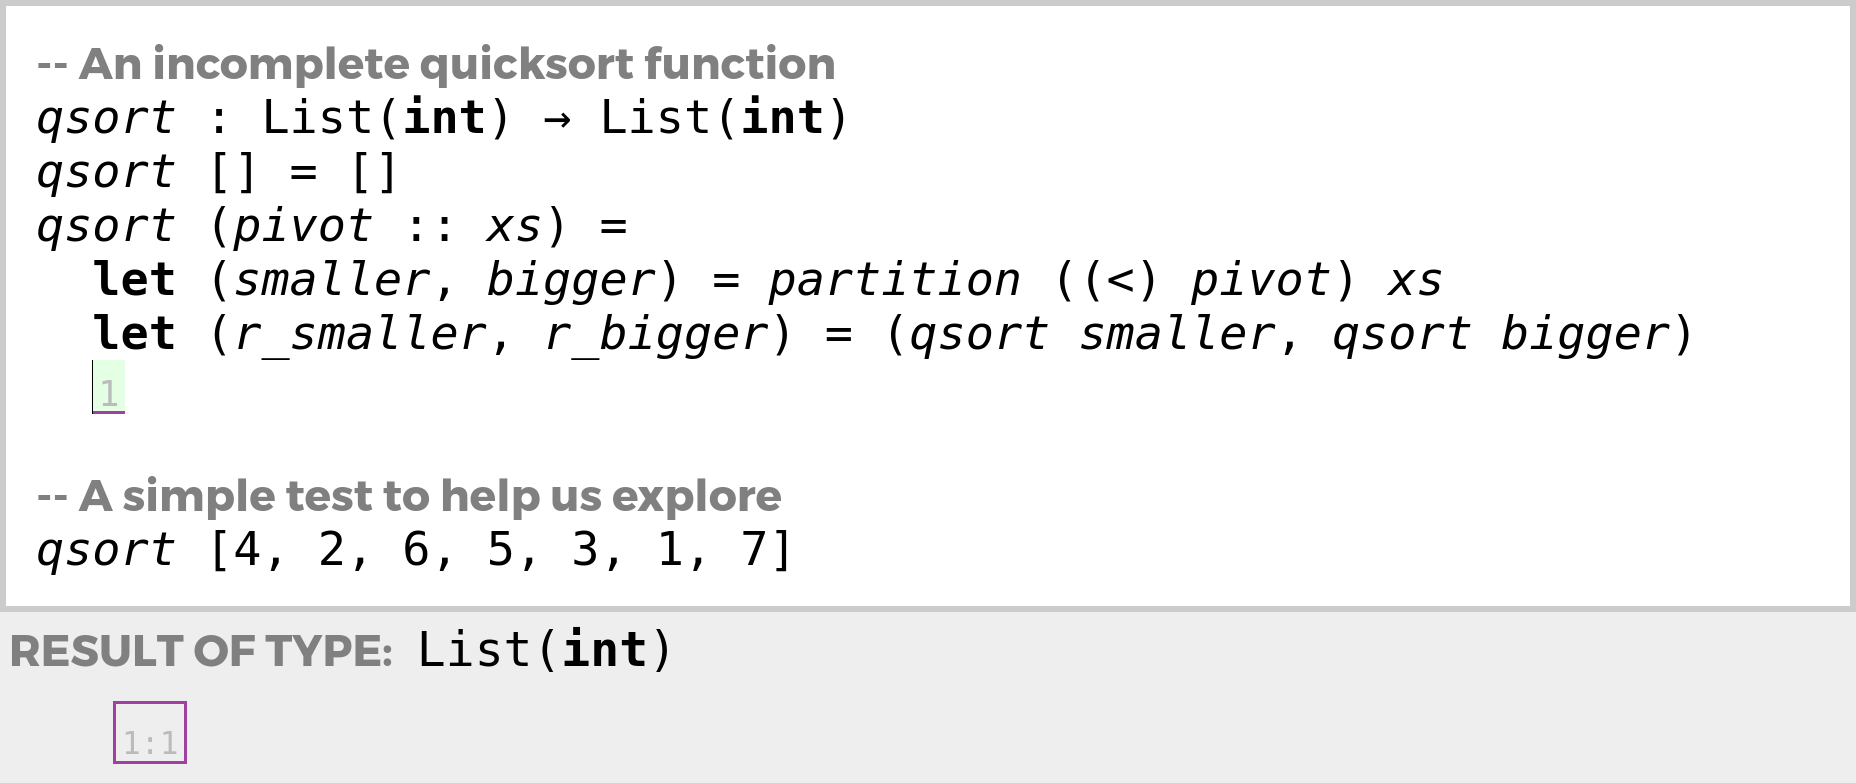
\includegraphics[width=\textwidth,interpolate=false,valign=t]{images/qsort-code.png}
\caption{The result of evaluation is a hole closure.}
\label{fig:qsort-example-code}
\end{subfigure}
~
\begin{subfigure}[t]{0.33\textwidth}
\centering
\includegraphics[width=\textwidth,interpolate=false,valign=t]{images/type-inspector.png}
\vspace{-2px}
\caption{The type inspector
continuously provides static information about the expression at the cursor. Here, it tells us that the hole at the cursor should be filled by a list expression. Holes have hole (i.e. unknown) type.
}
\label{fig:qsort-type-inspector}
\end{subfigure}

\vspace{10px}

\begin{subfigure}[t]{\textwidth}
\centering
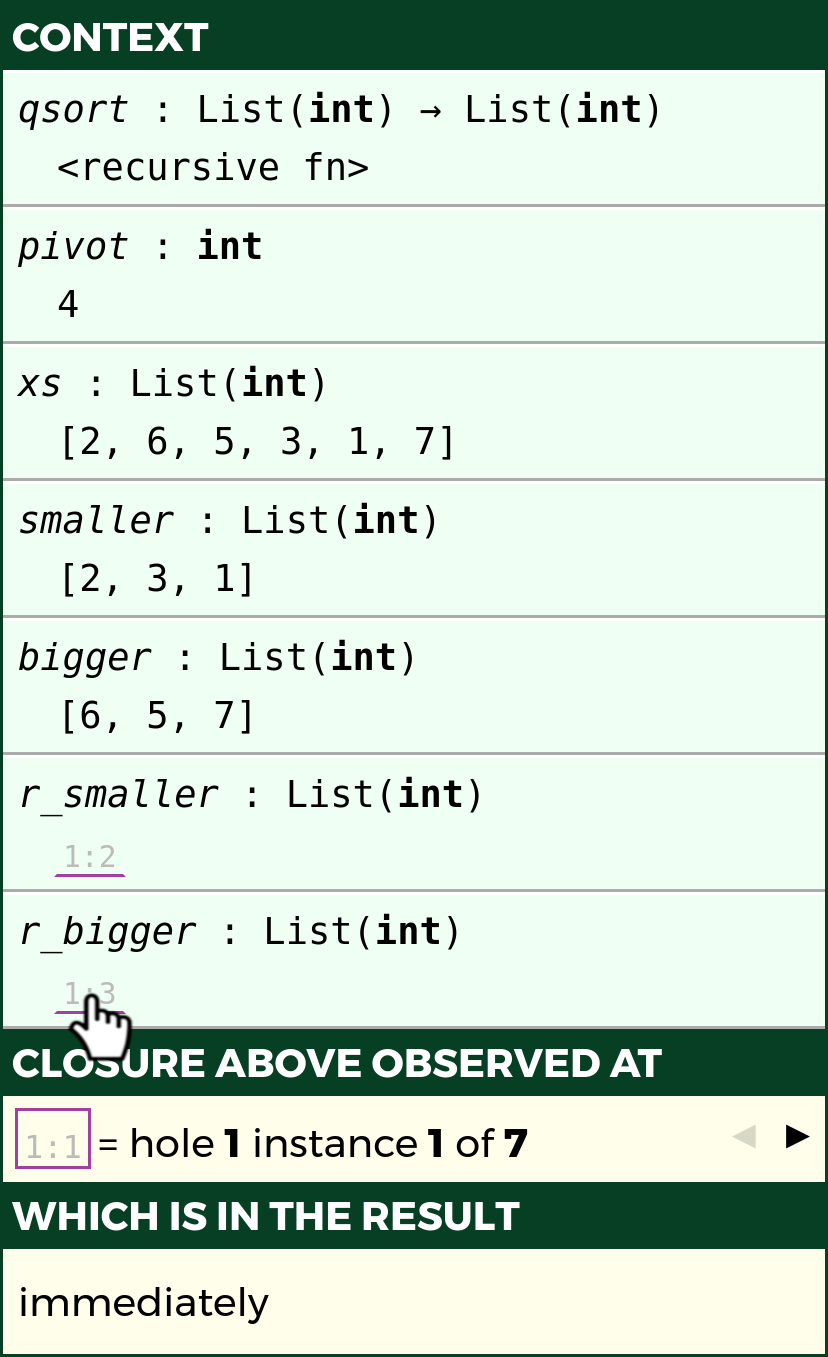
\includegraphics[width=0.29\textwidth,interpolate=false,valign=c]{images/qsort-new-sidebar-1.png}
~$\xrightarrow[\text{click}]{}$
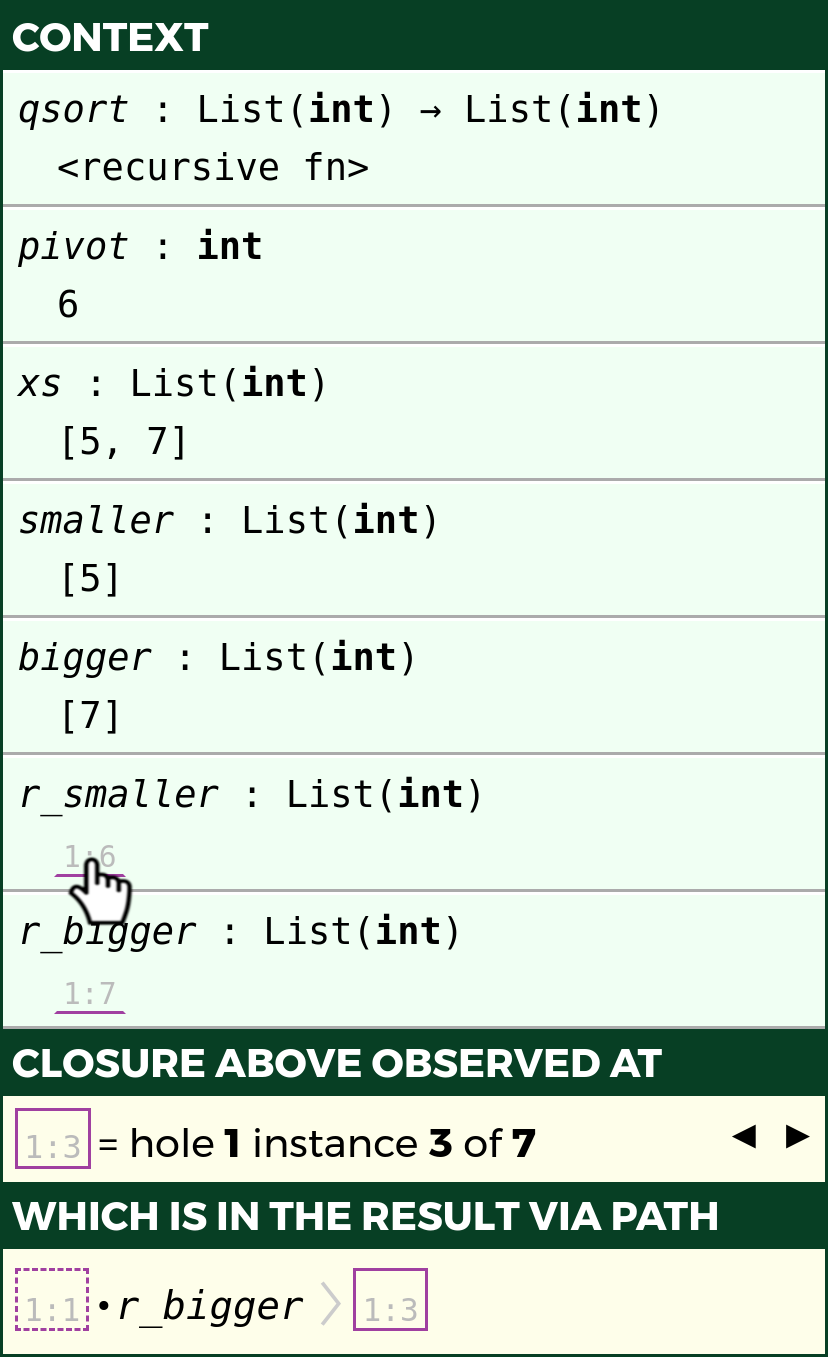
\includegraphics[width=0.29\textwidth,interpolate=false,valign=c]{images/qsort-new-sidebar-2.png}
~$\xrightarrow[\text{click}]{}$
\includegraphics[width=0.29\textwidth,interpolate=false,valign=c]{images/qsort-new-sidebar-3.png}
\caption{The programmer can explore the recursive structure of the computation by clicking on hole instances.}
\label{fig:qsort-sidebars}
\end{subfigure}

\vspace{3px}

\caption{Example 2: Incomplete Quicksort}
\label{fig:qsort-cell-mockup}
% \end{subfigure}

\vspace{-6px}
\end{figure}

% \begin{subfigure}[t]{\textwidth}
% \centering
% \includegraphics[width=0.3\textwidth,interpolate=false]{images/grades-sidebar-1.png}
% ~${}^\blacktriangleright$
% \includegraphics[width=0.3\textwidth,interpolate=false]{images/grades-sidebar-2.png}
% ~${}^\blacktriangleright$
% \includegraphics[width=0.3\textwidth,interpolate=false]{images/grades-sidebar-3.png}
% \caption{Typing context view with live hole closure information}
% \label{sec:grades-sidebar}
% \end{subfigure}
% %% TODO once the code above is removed, scale up the screenshots
% \includegraphics[scale=0.20]{images/hazel-placeholder-0.png}

% \rkc{Draw arrows and captions on the top figure to show how to get
% to the bottom figure.
% ser navigates to hole a, types + to create a plus, types * to create a
% multiplication, types \#10 to create 10, types vh1 to create variable use.}

% \includegraphics[scale=0.20]{images/hazel-placeholder-1a.png}
